% 第2章第3节：对偶空间（对偶空间与Hahn--Banach延拓、积分空间的对偶、连续函数空间与测度表示）。

\section{对偶空间}
\label{sec:lfo-dual}

上一节逐个研究读数规则，本节把同一空间上的全部有界线性读数收集成一个空间。我们关心两个问题：这些读数是否多到足以区分任意两个不同的元素，以及在具体的函数空间中，它们究竟长什么样。前一个问题由延拓定理回答，适用于一切赋范空间；后一个问题要按原空间的类型分别回答。

\subsection{对偶空间与泛函延拓}
\label{sec:lfo-hahn-banach}

\begin{definition}[对偶空间]
\label{def:lfo-dual-space}
赋范空间$X$上全部有界线性泛函组成的空间$X^*=\mathcal B(X,\mathbb F)$称为$X$的\term{对偶空间}（dual space），配以泛函范数$\|L\|=\sup_{\|x\|\leq1}|L(x)|$。
\end{definition}

标量域$\mathbb F$是完备的，所以由定理~\ref{thm:lfo-operator-space-complete}，无论$X$本身是否完备，$X^*$总是Banach空间。例如在不完备的多项式空间上配一致范数，它的对偶空间仍然完备。

\paragraph{读数规则与向量表示不是一回事}
对偶空间的元素是读数规则，不是原空间的元素。即使在有限维中，两者的范数也可能不同。在$\mathbb R^2$上配$\ell^1$范数$\|\bm x\|_1=|x_1|+|x_2|$，每个线性泛函都写成$L(\bm x)=a_1x_1+a_2x_2$。由$|L(\bm x)|\leq\max(|a_1|,|a_2|)\,\|\bm x\|_1$，且在$\bm x=\bm e_1$或$\bm e_2$处等号可以成立，得$\|L\|=\max(|a_1|,|a_2|)$。系数向量$\bm a$属于$\mathbb R^2$，但它作为读数的长度要用$\ell^\infty$范数计算，这是\term{对偶范数}（dual norm）的一个例子。

Hilbert空间是特殊情形：Riesz表示定理把每个读数对应到唯一的向量$h_L$，并且$\|L\|=\|h_L\|$，所以$H^*$与$H$可以通过保范数的（复情形下共轭线性的）双射视为同一个空间。对一般空间不能直接写$X^*=X$；第~\ref{sec:lfo-lp-dual}节会看到，$L^p$的对偶在$p\neq2$时由另一个空间$L^q$表示。

\paragraph{读数够不够区分元素}
在Hilbert空间中，若$x\neq0$，读数$\langle x,\cdot\rangle$在$x$处给出$\|x\|^2\neq0$，所以总有连续读数能把$x$与$0$区分开。一般的Banach空间没有内积，无法直接写出这样的读数。我们能做的是先在包含$x$的一维子空间上定义一个读数，再设法把它延拓到全空间，并且不增大它的范数。保证这种延拓存在的是\term{Hahn--Banach定理}（Hahn--Banach theorem）。

\begin{theorem}[Hahn--Banach定理（保范数延拓）]
\label{thm:lfo-hahn-banach}
设$X$是赋范空间，$M\subset X$是线性子空间，$\ell:M\to\mathbb F$是有界线性泛函。则存在$L\in X^*$，使$L|_M=\ell$且$\|L\|=\|\ell\|$。
\end{theorem}

\paragraph{延拓一维：可选范围非空}
以实空间为例看延拓的核心一步。不妨设$\|\ell\|=1$，任取$z\notin M$，要把$\ell$延拓到$M\oplus\operatorname{span}\{z\}$上。线性延拓完全由一个数$t=L(z)$决定：$L(m+sz)=\ell(m)+st$。要求$\|L\|\leq1$，即$|\ell(m)+st|\leq\|m+sz\|$对一切$m\in M$、$s\in\mathbb R$成立。$s=0$时这就是$\|\ell\|\leq1$；$s\neq0$时两边除以$|s|$并把$m/s$重新记为$m$，条件化为
\[
 -\|m+z\|-\ell(m)\leq t\leq\|m+z\|-\ell(m)\qquad(m\in M).
\]
这样的$t$存在，当且仅当左端对$m$的上确界不超过右端对$m'$的下确界，即对一切$m,m'\in M$，
\[
 -\|m+z\|-\ell(m)\leq\|m'+z\|-\ell(m') .
\]
这确实成立，因为$\ell(m')-\ell(m)=\ell(m'-m)\leq\|m'-m\|\leq\|m'+z\|+\|m+z\|$，移项即得。所以可选的$t$组成一个非空区间，任取其中一个就把$\ell$保范数地延拓了一维。

\paragraph{从一维到全空间（补充）}
若$X$可分，取可数稠密集$\{z_1,z_2,\ldots\}$，逐个把$z_k$添进定义域并重复上面的一步，就把$\ell$保范数地延拓到$\operatorname{span}(M\cup\{z_k\})$上；这个子空间稠密，延拓后的泛函一致连续，可以唯一地连续延拓到整个$X$，范数不变。不可分时，“逐个添加”需要用Zorn引理代替归纳法，思路相同。复空间的情形可以先延拓实部$\operatorname{Re}\ell$，再由$L(x)=\operatorname{Re}L(x)-i\operatorname{Re}L(ix)$恢复复线性泛函。这些细节属于补充，主线只需记住条件（$\ell$在子空间上有界）和结论（全空间上存在范数相同的延拓）。

\paragraph{延拓可以不唯一}
图~\ref{fig:lfo-hahn-banach}展示了一维延拓中的那个“非空区间”。在$(\mathbb R^2,\|\cdot\|_1)$中取$M$为横轴，$\ell(s,0)=s$，$\|\ell\|=1$。延拓为$L_t(\bm x)=x_1+tx_2$，由前面对偶范数的计算，$\|L_t\|=\max(1,|t|)$，所以$|t|\leq1$的每个$t$都给出保范数延拓。几何上，水平线$\{L_t=1\}$都经过点$(1,0)$并支撑菱形单位球；菱形在这个顶点处有许多支撑线，延拓因而不唯一。在欧氏范数下，单位圆在$(1,0)$只有一条切线$x_1=1$，延拓唯一。一般地，Hilbert空间中的保范数延拓是唯一的，就是$L=\ell\circ P_{\overline M}$（$\ell$先连续延拓到闭包$\overline M$上）。

\begin{figure}[!htb]
  \centering
  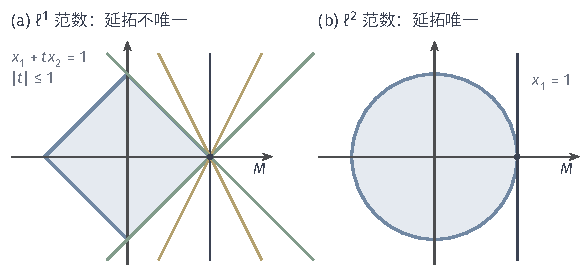
\includegraphics[width=98.9mm]{figures/02-abstract-mathematics/03-function-spaces/tikz/c2-hahn-banach/figure.pdf}
  \caption{保范数延拓与单位球的支撑线。(a)~$(\mathbb R^2,\|\cdot\|_1)$的单位球是菱形，子空间$M$为横轴，$\ell(s,0)=s$。延拓$L_t(\bm x)=x_1+tx_2$在$|t|\leq1$时范数都为$1$，对应的水平线$x_1+tx_2=1$（图中$t=0,\pm\frac12,\pm1$）都过$(1,0)$并支撑菱形；(b)~欧氏单位圆在$(1,0)$只有一条支撑线$x_1=1$，保范数延拓唯一。}
  \label{fig:lfo-hahn-banach}
\end{figure}

\paragraph{读数足以区分元素}
把定理用于一维子空间，就得到本小节开头的问题的答案。

\begin{theorem}[范数的对偶刻画]
\label{thm:lfo-norming-functional}
设$X$是赋范空间，$x\in X$且$x\neq0$。则存在$L\in X^*$，使$\|L\|=1$且$L(x)=\|x\|$。因此对一切$x\in X$，
\begin{equation}
 \|x\|=\sup_{\|L\|\leq1}|L(x)|=\max_{\|L\|\leq1}|L(x)| ,
 \label{eq:lfo-norm-dual}
\end{equation}
并且若$L(x)=L(z)$对一切$L\in X^*$成立，则$x=z$。
\end{theorem}

\begin{proof}
在$M=\operatorname{span}\{x\}$上令$\ell(\alpha x)=\alpha\|x\|$，则$|\ell(\alpha x)|=\|\alpha x\|$，$\|\ell\|=1$。由定理~\ref{thm:lfo-hahn-banach}延拓得到所需的$L$。对一切$\|L'\|\leq1$有$|L'(x)|\leq\|x\|$，而上面的$L$取到等号，故式~\eqref{eq:lfo-norm-dual}成立（$x=0$时两边为零）。最后，若$x\neq z$，对$x-z$取这样的$L$，得$L(x)-L(z)=\|x-z\|\neq0$。
\end{proof}

式~\eqref{eq:lfo-norm-dual}说，一个元素的长度可以由单位读数的最大读值完全恢复。在具体空间中，取到最大值的读数常常可以直接写出。例如在$C([0,1])$中，设$|f|$在$t_0$处取到最大值，则$L=\operatorname{sgn}(f(t_0))\,\delta_{t_0}$就满足$\|L\|=1$、$L(f)=\|f\|_\infty$。定理的价值在于，即使写不出这样的读数，它也保证存在。

凸集的分离、优化问题的对偶以及最优性条件，都是同一延拓思想的几何形式，属于优化问题，可参考\BookChapterRef{chap:constrained-optimization}{卷三“有约束优化的求解”章}。

\subsection{积分空间的对偶}
\label{sec:lfo-lp-dual}

第~\ref{sec:lfo-point-evaluation}节用Hölder不等式说明，每个$g\in L^q$都给出$L^p$上的有界读数$L_g$。本小节回答反方向的问题：$L^p$上的每个有界读数是否都来自某个权重$g$，权重的范数又是否等于读数的范数。为避免共轭记号，先在实值函数上讨论，复情形在小节末交代。

\begin{theorem}[$L^p$的对偶]
\label{thm:lfo-lp-dual}
设$(\Omega,\mathcal F,\mu)$是$\sigma$有限测度空间，$1\leq p<\infty$，$q$为共轭指数。则映射$g\mapsto L_g$，$L_g(f)=\int_\Omega fg\,d\mu$，是从$L^q(\mu)$到$(L^p(\mu))^*$的保范数线性双射，即每个$L\in(L^p)^*$都唯一地写成$L=L_g$，且$\|L\|=\|g\|_q$。
\end{theorem}

证明分两部分：正向说明$\|L_g\|$恰好等于$\|g\|_q$，反向说明每个读数都有这样的权重。

\paragraph{正向：等号由哪个输入取到}
Hölder不等式已给出$\|L_g\|\leq\|g\|_q$，只需找输入取到或逼近等号。设$1<p<\infty$，$g\neq0$。令$f=|g|^{q-1}\operatorname{sgn}(g)$，则$fg=|g|^q$，并且$|f|^p=|g|^{(q-1)p}=|g|^q$（因为$(q-1)p=q$）。于是
\[
 \begin{aligned}
 &L_g(f)=\int|g|^q\,d\mu=\|g\|_q^q,\qquad \|f\|_p=\|g\|_q^{q/p},\\
 &\frac{L_g(f)}{\|f\|_p}=\|g\|_q^{\,q-q/p}=\|g\|_q .
 \end{aligned}
\]
$p=1$、$q=\infty$时等号未必取到，改用逼近：对$\varepsilon>0$，集合$E=\{|g|>\|g\|_\infty-\varepsilon\}$测度为正；由$\sigma$有限，可取$E$中测度有限且为正的部分$E'$，令$f=\operatorname{sgn}(g)\mathbf 1_{E'}/\mu(E')$，则$\|f\|_1=1$而$L_g(f)\geq\|g\|_\infty-\varepsilon$。正向保范数说明映射$g\mapsto L_g$单射。

\paragraph{反向：由读数生成测度}
先设$\mu$有限。给定$L\in(L^p)^*$，对可测集$E$令$\nu(E)=L(\mathbf 1_E)$。证明$\nu$是有限符号测度并对$\mu$绝对连续，就可以调用Radon--Nikodym定理。

有限可加性来自$L$的线性：不交时$\mathbf 1_{E\cup F}=\mathbf 1_E+\mathbf 1_F$。可数可加性来自$L$的连续性，这里用到$p<\infty$：若$E=\bigcup_kE_k$为不交并，则
\[
 \Bigl\|\mathbf 1_E-\sum_{k\leq n}\mathbf 1_{E_k}\Bigr\|_p=\mu\Bigl(\bigcup_{k>n}E_k\Bigr)^{1/p}\longrightarrow0 ,
\]
所以$\sum_{k\leq n}\nu(E_k)\to\nu(E)$。绝对连续性同样直接：$\mu(E)=0$时$\mathbf 1_E$是$L^p$中的零元，$\nu(E)=L(0)=0$。由第~\ref{sec:measure-signed-total-variation}节的Jordan分解（定理~\ref{thm:measure-hahn-jordan}），$\nu$是两个有限测度之差，二者都对$\mu$绝对连续；分别应用Radon--Nikodym定理（定理~\ref{thm:measure-radon-nikodym}），得到可积函数$g$使
\[
 L(\mathbf 1_E)=\int_Eg\,d\mu\qquad(E\in\mathcal F).
\]

\paragraph{反向：从示性函数推广到全空间}
由线性，$L(f)=\int fg\,d\mu$对简单函数$f$成立。接下来说明$g\in L^q$，并把等式推广到全部$L^p$。对$1<p<\infty$，令$E_n=\{|g|\leq n\}$，$f_n=|g|^{q-1}\operatorname{sgn}(g)\mathbf 1_{E_n}$。$f_n$是有界可测函数，可由简单函数一致逼近；在有限测度下一致收敛蕴含$L^p$收敛，两端都随之收敛，所以等式对$f_n$也成立。于是
\[
 \int_{E_n}|g|^q\,d\mu=L(f_n)\leq\|L\|\,\|f_n\|_p=\|L\|\Bigl(\int_{E_n}|g|^q\,d\mu\Bigr)^{1/p},
\]
整理得$(\int_{E_n}|g|^q)^{1/q}\leq\|L\|$。令$n\to\infty$，由单调收敛定理，$\|g\|_q\leq\|L\|$。$p=1$时可类似地在$\{|g|>\|L\|\}$上取示性函数说明该集合零测。既然$g\in L^q$，$L$与$L_g$都是$L^p$上的连续泛函，又在简单函数上相等；第~\ref{sec:fs-density-separability}节说明简单函数在$L^p$中稠密，所以$L=L_g$。

\paragraph{$\sigma$有限情形（补充）}
一般的$\sigma$有限测度把$\Omega$分成可数个测度有限的不交片$\Omega_k$。在每一片上得到$g_k$，由唯一性它们彼此相容，拼成$g=\sum_kg_k\mathbf 1_{\Omega_k}$；对每个有限并的范数估计都不超过$\|L\|$，再用单调收敛得$\|g\|_q\leq\|L\|$。$p=1$时$\sigma$有限不能去掉，$1<p<\infty$时则可以用更细的论证去掉这一假设，这里不展开。

\paragraph{复值函数的配对}
复值情形下，为与内积约定一致，把配对写成$L_g(f)=\int\bar gf\,d\mu$，即对权重取共轭、对输入线性。$p=2$时它正是$\langle g,f\rangle$，定理~\ref{thm:lfo-lp-dual}回到Riesz表示定理。正向构造中的$\operatorname{sgn}(g)$相应换为$g/|g|$（$g=0$处取零）。

\paragraph{一个可复算的范数}
在$L^3(0,1)$上取读数$L(f)=\int_0^1tf(t)\,dt$。共轭指数$q=3/2$，由定理~\ref{thm:lfo-lp-dual}，
\[
 \|L\|=\|t\|_{3/2}=\Bigl(\int_0^1t^{3/2}\,dt\Bigr)^{2/3}=\Bigl(\frac25\Bigr)^{2/3}\approx0.543 ,
\]
取到范数的输入是$f(t)=t^{q-1}=t^{1/2}$。同一个权重在$L^2$中的读数范数是$\|t\|_2=1/\sqrt3\approx0.577$，在$L^1$中是$\|t\|_\infty=1$：指数$p$越小，$L^p$范数对集中在小区域上的输入越宽容，读数相对于它的放大就可能越大。

\paragraph{端点：$L^\infty$的对偶更大}
定理排除了$p=\infty$，这不是技术上的疏漏。$L^1$的对偶是$L^\infty$，但$L^\infty$的对偶一般不能全部由$L^1$表示。以计数测度下的$\ell^\infty$为例。在收敛数列组成的子空间$c$上定义$\ell(x)=\lim_nx_n$，它的范数为$1$。由Hahn--Banach定理，它延拓为某个$L\in(\ell^\infty)^*$。若$L$由某个$g\in\ell^1$表示，即$L(x)=\sum_kg_kx_k$，则由标准单位向量满足$L(e_k)=\lim_n(e_k)_n=0$得每个$g_k=0$，于是$L=0$；可是$L$在常数列$(1,1,\ldots)$上的值为$1$，矛盾。所以$(\ell^\infty)^*$严格大于$\ell^1$；对Lebesgue测度下的$L^\infty(0,1)$也有类似的构造。

这一端点限制为第~\ref{sec:lfo-reflexive}节的反射性和第~\ref{sec:lfo-weak-star}节的弱星收敛保留了准确的入口。有限维和$L^2$中“对偶就是自身”的直觉，不能直接推广到所有积分空间。

\subsection{连续函数空间与测度表示（补充）}
\label{sec:lfo-ck-dual}

本小节转到另一类空间$C(K)$，其中$K$是紧致度量空间，配一致范数，只考虑实值函数。它的读数不再总能写成权重函数的积分，而要用测度表示，相应的结论称为\term{Riesz--Markov--Kakutani表示定理}（Riesz--Markov--Kakutani representation theorem）。

\paragraph{几种读数都是对测度积分}
先看$C([0,1])$上的几个读数：点值$f(0)$，平均$\int_0^1f\,dt$，两者之和，以及端点差$f(1)-f(0)$。它们分别是对测度$\delta_0$、Lebesgue测度$\lambda$、$\delta_0+\lambda$和$\delta_1-\delta_0$的积分，其中$\delta_x$是集中在$x$处的单位质量，称为\term{Dirac测度}（Dirac measure）。一般地，对有限符号Borel测度$\mu$，读数$f\mapsto\int_Kf\,d\mu$满足
\[
 \Bigl|\int_Kf\,d\mu\Bigr|\leq\int_K|f|\,d|\mu|\leq\|f\|_\infty\,|\mu|(K),
\]
其中$|\mu|$是第~\ref{sec:measure-signed-total-variation}节的全变差测度。以端点差为例，$|\mu|(K)=2$，取$f(t)=2t-1$得读数$2$而$\|f\|_\infty=1$，所以读数范数恰为$2$。

\begin{theorem}[$C(K)$的对偶（Riesz--Markov--Kakutani）]
\label{thm:lfo-ck-dual}
设$K$是紧致度量空间。对每个$L\in C(K)^*$，存在唯一的有限符号正则Borel测度$\mu$，使$L(f)=\int_Kf\,d\mu$对一切$f\in C(K)$成立，并且$\|L\|=|\mu|(K)$。
\end{theorem}

\paragraph{证明思路（补充）}
先处理正读数，即$f\geq0$时$L(f)\geq0$的读数。对开集$U$，用$L$在$0\leq f\leq1$且支撑在$U$内的连续函数上的上确界定义$\mu(U)$，再由开集向一般Borel集延拓；正性保证得到的是正测度，连续函数可以从内部逼近开集的示性函数，这保证了$\int f\,d\mu=L(f)$。一般读数分解为两个正读数之差：对$f\geq0$令$L^+(f)=\sup\{L(u):0\leq u\leq f\}$，再线性延拓，则$L^-=L^+-L$也是正读数，两者分别对应测度$\mu^+$、$\mu^-$。在紧致度量空间中，有限Borel测度自动是正则的，正则性保证了表示的唯一性。完整证明见泛函分析教材，主线只使用定理的结论。

\paragraph{测度不必有密度}
表示$C(K)$上读数的是测度，而不是权重函数。点值$\delta_x$对Lebesgue测度没有密度：第~\ref{sec:measure-same-space-comparison}节已经说明，单点质量不能写成“在一点处取无穷大的密度函数”。所以不能把定理~\ref{thm:lfo-ck-dual}理解为“每个读数都有逐点权重”，权重函数只在测度对参考测度绝对连续时才存在。

\paragraph{同一个读数，三种表示}
“读出一点的值”在三种空间中得到三种不同的待遇。在$C(K)$中，它是Dirac测度$\delta_x$，是对偶空间中范数为$1$的元素；在$L^2$中，它根本没有良定义；在第~\ref{chap:rkhs}章的再生核Hilbert空间中，它是有界读数，由Riesz表示对应到一个函数方向$K_x$。表示的形式取决于空间的结构，而不取决于读数规则的文字描述。

\paragraph{与测度弱收敛的关系}
定理~\ref{thm:lfo-ck-dual}把$C(K)^*$与$K$上的有限符号测度等同起来。第~\ref{sec:measure-sequence-convergence}节的概率测度弱收敛要求$\int f\,d\mu_n\to\int f\,d\mu$对一切有界连续$f$成立；在紧致的$K$上，这正是第~\ref{sec:lfo-weak-star}节将要定义的$C(K)^*$中的弱星收敛。测度的弱收敛已有独立的定义和基础，不需要先掌握这里的一般表示定理；本小节只是指出两者在紧致空间上的对应。概率分布之间更细致的比较属于后续问题，可参考\BookChapterRef{chap:information-theory-and-statistical-geometry}{卷四“概率分布的分析与优化”章}。
